\documentclass{article}
\usepackage{ctex}
\usepackage{amsmath}
\usepackage{graphicx}


\title{机器学习作业3}
\begin{document}
\maketitle
\begin{center}
181860152 周宇翔
\end{center}
\section*{1.[20pts]Decision Tree}\noindent
\subsection*{(1)}\noindent
f是realizable的\\
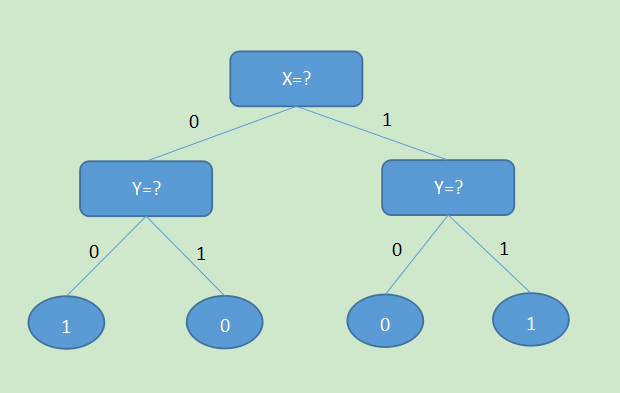
\includegraphics[scale=0.5]{tree.png}
\subsection*{(2)}\noindent
$p_0=0.4,p_1=0.6$\\
$Ent(D)=-\sum_{k=0}^{1}p_klog_2p_k\\
=-0.4log_20.4-0.6log_20.6=0.971$\\
设两个Feature分别为$F_1,F_2$($F_1,F_2$就是$x_1,x_2$我后来才发现但是懒得改了ovo)\\
如果把$F_1,F_2$按照离散值处理:
$Gain(D,F_1)=Ent(D)-10*\frac{1}{10}*0=0.971\\
IV(a)=log_2{10}=3.32\\
Gain\_ratio(D,F_1)=0.292$\\
类似的$Gain\_ratio(D,F_2)=0.292$\\
但是如果把每个feature当作离散值的一个分类处理,会导致虽然每个节点的纯度很高,但是决策树的泛化能力很弱,无法对新样本进行有效预测\\
因此应该把这些值当作连续值处理\\
划分点选取:首先选取$F_1$作为划分属性,连续值排序后为22,23,24,25,32,43,48,52,52,53\\
候选划分点为\{22.5,23.5,24.5,28.5,37.5,45.5,50,52,52.5\}\\
$Gain(D,F_1,22.5)=0.971-0-\frac{9}{10}(-\frac{4}{9}log_2\frac{4}{9}-\frac{5}{9}log_2\frac{5}{9})=0.079\\
Gain(D,F_1,23.5)=0.971+0.2*2*0.5log_20.5+0.8*(\frac{3}{8}log_2\frac{3}{8}+\frac{5}{8}log_2\frac{5}{8})=7.45*10^{-3}\\
Gain(D,F_1,24.5)=0.971+0.3(\frac{1}{3}log_2\frac{1}{3}+\frac{2}{3}log_2\frac{2}{3})+0.7(\frac{4}{7}log_2\frac{4}{7}+\frac{3}{7}log_2\frac{3}{7})=5.85*10^{-3}\\
Gain(D,F_1,28.5)=0.971+0.4(\frac{1}{4}log_2\frac{1}{4}+\frac{3}{4}log_2\frac{3}{4})+0.6(2*\frac{1}{2}log_2\frac{1}{2})=0.0465\\
Gain(D,F_1,37.5)=0.971+0.5(\frac{1}{5}log_2\frac{1}{5}+\frac{4}{5}log_2\frac{4}{5})+0.5(\frac{2}{5}log_2\frac{2}{5}+\frac{3}{5}log_2\frac{3}{5})=0.124\\
Gain(D,F_1,45.5)=0.971+0.6(\frac{1}{3}log_2\frac{1}{3}+\frac{2}{3}log_2\frac{2}{3})+0.4*2*\frac{1}{2}*log_2\frac{1}{2}=0.0200\\
Gain(D,F_1,50)=0.971+0.7(\frac{2}{7}log_2\frac{2}{7}+\frac{5}{7}log_2\frac{5}{7})+0.3(\frac{1}{3}log_2\frac{1}{3}+\frac{2}{3}log_2\frac{2}{3})=0.0913\\
Gain(D,F_1,52)=Gain(D,F_1,52.5)=0.971+0.9(\frac{2}{3}log_2\frac{2}{3}+\frac{1}{3}log_2\frac{1}{3})=0.145\\$
\\
选取$F_2$作为划分属性,连续值排序后为25,27,38,40,44,48,52,65,77,110\\
候选划分点为\{26,32.5,39,42,46,50,58.5,71,93.5\}\\
$Gain(D,F_2,26)=0.971+0.9(\frac{2}{3}log_2\frac{2}{3}+\frac{1}{3}log_2\frac{1}{3})=0.0527\\
Gain(D,F_2,32.5)=0.971+0.8(\frac{1}{4}log_2\frac{1}{4}+\frac{3}{4}log_2\frac{3}{4})=0.322\\
Gain(D,F_2,39)=0.971+0.3(\frac{1}{3}log_2\frac{1}{3}+\frac{2}{3}log_2\frac{2}{3})+0.7(\frac{5}{7}log_2\frac{5}{7}+\frac{2}{7}log_2\frac{2}{7})=0.0913\\
Gain(D,F_2,42)=0.971+0.4*2*\frac{1}{2}log_2\frac{1}{2}+0.6(\frac{1}{3}log_2\frac{1}{3}+\frac{2}{3}log_2\frac{2}{3})=0.0200\\
Gain(D,F_2,46)=0.971+0.5(\frac{2}{5}log_2\frac{2}{5}+\frac{3}{5}log_2\frac{3}{5})+0.5(\frac{1}{5}log_2\frac{1}{5}+\frac{4}{5}log_2\frac{4}{5})=0.124\\$
$Gain(D,F_2,50)=0.971+0.6(\frac{1}{2}log_2\frac{1}{2}*2)+0.4(\frac{1}{4}log_2\frac{1}{4}+\frac{3}{4}log_2\frac{3}{4})=0.146\\
Gain(D,F_2,58.5)=0.971+0.7(\frac{3}{7}log_2\frac{3}{7}+\frac{4}{7}log_2\frac{4}{7})=0.281\\
Gain(D,F_2,71)=0.971+0.8(2*\frac{1}{2}\frac{1}{2})=0.171\\
Gain(D,F_2,93.5)=0.971+0.9(\frac{4}{9}log_2\frac{4}{9}+\frac{5}{9}log_2\frac{5}{9})=0.079$\\
综合选取使得Gain(D,a,t)为Gain(D,$F_2$,32.5),也即第一步采用$F_2$划分,分界点为32.5\\
再根据$F_1$进行划分,对于$F_2<=32.5$的情况已经无需再划分,对于$F_2>32.5$的情况,$F_1$的取值排序后为22,24,25,32,43,48,52,53\\
候选划分点为\{23,24.5,28.5,37.5,45.5,50,52.5\}\\
$Gain(D,F_1,23)-Ent(D)=\frac{7}{8}(\frac{5}{7}log_2\frac{5}{7}+\frac{2}{7}log_2\frac{2}{7})=-0.755\\
Gain(D,F_1,24.5)-Ent(D)=\frac{3}{4}(\frac{1}{3}log_2\frac{1}{3}+\frac{2}{3}log_2\frac{2}{3})=-0.68\\
Gain(D,F_1,28.5)-Ent(D)=\frac{5}{8}(\frac{2}{5}log_2\frac{2}{5}+\frac{3}{5}log_2\frac{3}{5})=-0.607\\
Gain(D,F_1,37.5)-Ent(D)=\frac{1}{2}(\frac{1}{4}log_2\frac{1}{4}+\frac{3}{4}log_2\frac{3}{4})=-0.406\\
Gain(D,F_1,45.5)-Ent(D)=\frac{3}{8}(\frac{1}{3}log_2\frac{1}{3}+\frac{2}{3}log_2\frac{2}{3})+\frac{5}{8}(\frac{1}{5}log_2\frac{1}{5}+\frac{4}{5}log_2\frac{4}{5})=-0.796\\
Gain(D,F_1,50)-Ent(D)=\frac{1}{4}(\frac{1}{2}log_2\frac{1}{2}*2)+\frac{3}{4}(\frac{5}{6}log_2\frac{5}{6}+\frac{1}{6}log_2\frac{1}{6})=-0.738\\
Gain(D,F_1,52.5)-Ent(D)=\frac{7}{8}(\frac{6}{7}log_2\frac{6}{7}+\frac{1}{7}log_2\frac{1}{7})=-0.518$\\
综上选取$F_1=37.5$作为一个划分点;
对于$F_1<=37.5$的情况已无需再划分,对于$F_1>37.5$的情况易观察到$F_2=52.5$是一个最佳划分点,综上决策树如下\\
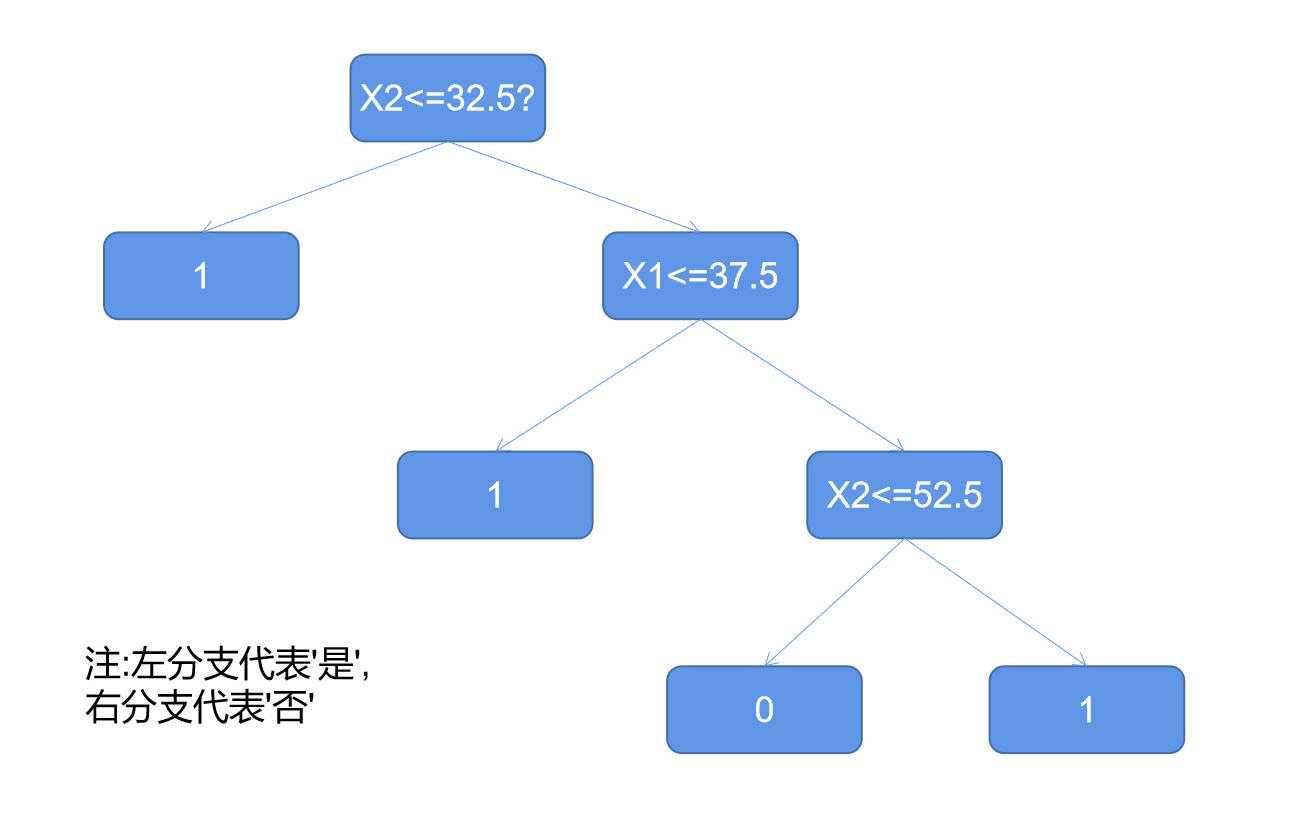
\includegraphics[scale=0.25]{DecTree.png}
\section*{2.[20pts]Neural Network}\noindent
\subsection*{(1)}\noindent
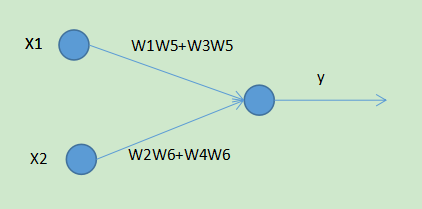
\includegraphics[scale=0.7]{redesign.png}
\subsection*{(2)}\noindent
可以,因为在这个计算过程中始终只会有输入变量$X_1,...,X_d$的一次项和常数项存在,不会产生交叉项,高次项或者非线性项,因此可以不用隐层表示
\subsection*{(3)}\noindent
对于Logistic Regression,输入$\textbf{X}={X_1,...,X_d}$\\
输出为$z=\textbf{w}^TX+b$,并用sigmoid函数$y=\frac{1}{1+e^{-z}}$来将z值转化为一个接近0或1的y值\\
对于含有隐层的神经网络,设置隐层同样含有d个神经元,输出记为$H_1,H_2,...,H_d$,第i个输入$X_i$和第j个隐层神经元$H_j$之间的权重设为$a_{ij}$,隐层采用线性激励函数$f(x)=x$,此时有如下关系\\
\begin{equation}
	\begin{bmatrix}
	a_{11}&...&a_{d1}\\
	...&&...\\
	a_{1d}&...&a_{dd}\\
	\end{bmatrix}
	{\begin{bmatrix}
	X_1,...,X_d
	\end{bmatrix}}^T=
	\begin{bmatrix}
	H_1,...,H_d
	\end{bmatrix}^T
\end{equation}\\
设第i个隐层神经元和输出神经元之间连接的权重为$w_i$,输出激励函数选取为sigmoid函数,阈值记作b\\
此时有\\
\begin{equation}
	z=
	\begin{bmatrix}
	H_1,...,H_d
	\end{bmatrix}
	\begin{bmatrix}
	w_1,...,w_d
	\end{bmatrix}^T-b
\end{equation}\\
\begin{equation}
	y=\frac{1}{1+e^{-z}}
\end{equation}\\
综合(1)式(2)式有
\begin{equation}
z=
\begin{bmatrix}
	a_{11}&...&a_{d1}\\
...&&...\\
a_{1d}&...&a_{dd}\\
\end{bmatrix}
{\begin{bmatrix}
	X_1,...,X_d
	\end{bmatrix}}^T
\begin{bmatrix}
w_1,...w_d
\end{bmatrix}^T-b
\\=\sum_{i=1}^{d}(\sum_{j=1}^{d}w_ja_{ij}X_i)-b
\end{equation}\\
根据看到此时的z和我们所要求得对数几率回归中的z是同一形式,在神经网络训练完成后,只要按照(4)式进行计算即可得到对应的对数几率回归的z函数的系数
\section*{3.[60pts]Neural Network in Practice}\noindent
\subsection*{(2)}\noindent
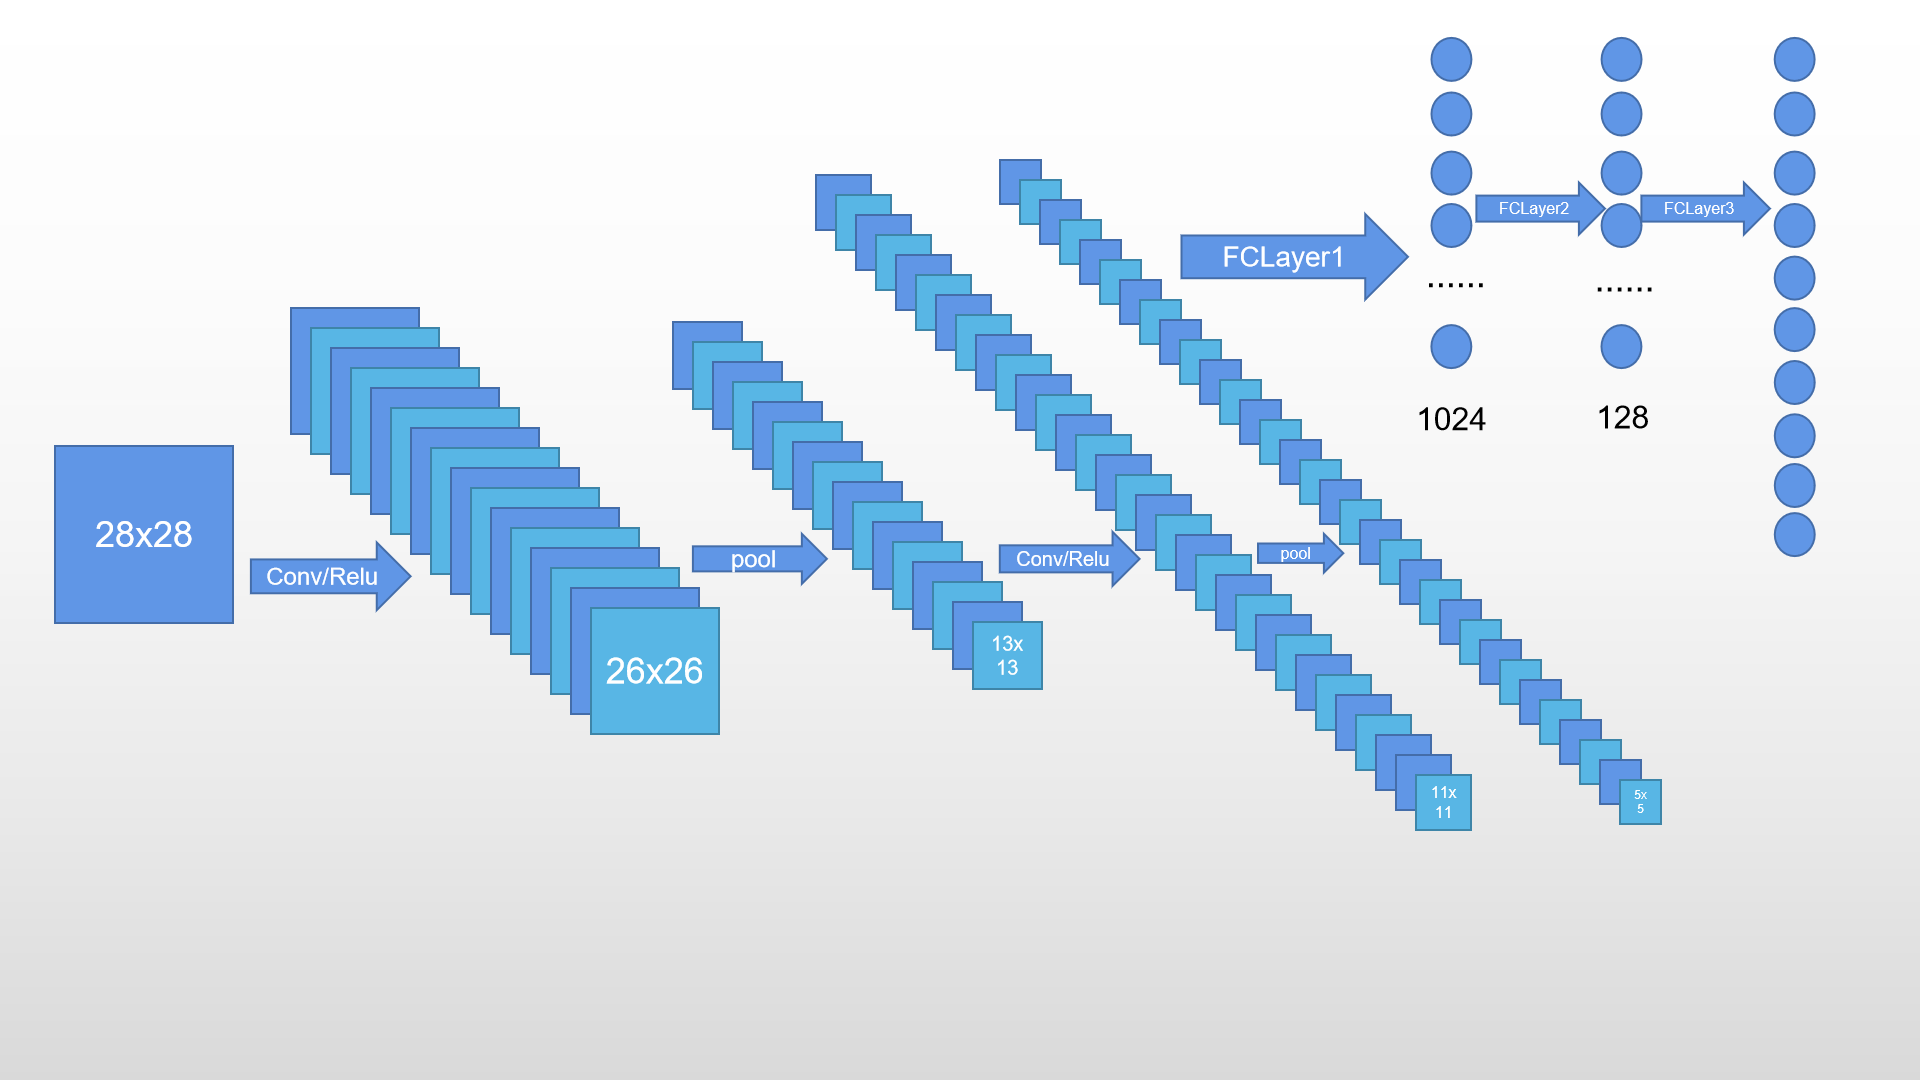
\includegraphics[scale=0.23]{Lenet.png}
\subsection*{(3)}\noindent
选取epochs$\in$\{1,2,3,4,5,6,7,8\},Learning Rate$\in$\{0.001,0.002,0.003,0.004,0.005\}进行测试\\
具体数据见附表params2.txt\\
综合Accuracy,AverageLoss以及Epochs考虑,选取\\
Epochs=7,Learning Rate=0.002进行作为该模型的参数
\subsection*{(4)}\noindent
对于training\_loss的变化,我采用对每一批(60个)数据都记录一次loss来刻画,并使用\\matplotlib.pylab来绘制图像\\
图大致如下,具体可见附件training\_loss.png\\
\includegraphics*[scale=0.33]{training_loss.png}
\end{document}